\documentclass[svgnames]{beamer}


\mode<presentation>
{
  \usetheme[titleformat=smallcaps,numbering=fraction,progressbar=frametitle]{metropolis}
  \usecolortheme[light,accent=orange]{solarized}
  %\usecolortheme[named=Goldenrod]{structure}
  % or ...

  \setbeamercovered{transparent}
  % or whatever (possibly just delete it)
}


% \usepackage{mathtext}
\usepackage[utf8]{inputenc}
\usepackage[english,russian]{babel}
\usepackage{cmap}
\hypersetup{unicode=true}
\graphicspath{{images/}{slides/images}}


\title[CMTA 03] % (optional, use only with long paper titles)
{Contrastive analysis}

\subtitle
{Computational Methods for Text Analysis} % (optional)

\author%[Author, Another] % (optional, use only with lots of authors)
{Кирилл Александрович Маслинский}
% - Use the \inst{?} command only if the authors have different
%   affiliation.

\institute%[Universities of Somewhere and Elsewhere] % (optional, but mostly needed)
{НИУ ВШЭ Санкт-Петербург}
% - Use the \inst command only if there are several affiliations.
% - Keep it simple, no one is interested in your street address.

\date%[Short Occasion] % (optional)
{25.09.2021 / 03}

\subject{natural language processing, text mining}
% This is only inserted into the PDF information catalog. Can be left
% out. 


\AtBeginSubsection[]
{
  \begin{frame}<beamer>[plain]{План}
    \tableofcontents[sectionstyle=show/hide,subsectionstyle=show/shaded/hide]
  \end{frame}
}

\newcommand{\tb}[1]{\colorbox{yellow}{#1}\space}
\newcommand{\Sp}[1]{\colorbox{green}{#1}\space}
\newcommand{\Sn}[1]{\colorbox{red}{#1}\space}


\begin{document}

\begin{frame}
  \titlepage
\end{frame}

\section{Ключевые слова}

\subsection{Использование контрастного корпуса}

\begin{frame}
  \frametitle{Метод контрастного корпуса}
  Задача — извлечение лексики, характерной для данного корпуса
  \begin{itemize}
  \item Контрастный корпус (reference corpus) — отражает
    словоупотребление в языке вообще или в более широкой предметной
    области
  \item Составить частотные списки слов для изучаемого и контрастного
    корпуса
  \item Отсортировать слова по расхождению частотности с ожидаемой
    на основании контрастного корпуса
  \item Ключевые слова изучаемого корпуса — наверху списка
  \end{itemize}
\end{frame}


\begin{frame}
  \frametitle{Ключевые слова корпуса}
  \begin{block}{Simple maths (by Adam Kilgarriff)}
  «это слово встречается в этом корпусе вдвое чаще, чем в том»
\end{block}
\begin{itemize}
\item Самый простой подход
  \begin{itemize}
  \item Нормализовать частотности
    \begin{itemize}
    \item употреблений на тысячу или употреблений на миллион (IPM)
    \end{itemize}
  \item Вычислить отношение нормализованных частотностей
  \item Отсортировать список слов по значению отношения
  \end{itemize}
\end{itemize}

Для примера: 
\begin{itemize}
\item Два корпуса по миллиону токенов
\item Нормализовать частотности не нужно
\item[Fc] focus corpus — изучаемый корпус
\item[Rc] reference corpus — контрастный корпус
\end{itemize}
\end{frame}

\begin{frame}
  \frametitle{Проблема 1:  нельзя делить на 0}
  \begin{tabular}[l]{lccc}
    слово & fc & rc & отношение \\
    \hline
    редкость & 10 & 0 &  ? \\
    помешивать & 100 & 0 &  ? \\
    вкуснотища & 1000 & 0 &  ? \\
  \end{tabular}

Стандартное решение: прибавить 1:

  \begin{tabular}[l]{lccc}
    слово & fc & rc & отношение \\
    \hline
    редкость & 11 & 1 &  11 \\
    помешивать & 101 & 1 &  101 \\
    вкуснотища & 1001 & 1 &  1001 \\
  \end{tabular}
\end{frame}

\begin{frame}
  \frametitle{Проблема 2: из-за редких слов слишком много больших
    отношений}
  Частотность тоже важна.   Решение: прибавить n.

  \begin{itemize}
  \item $n=1$

  \begin{tabular}[l]{lcccccc}
    слово & fc & rc & fc+n & rc+n & отношение & ранг \\
    \hline
    изредка & 10 & 0 & 11 & 1 & 11,00 & 1 \\
    временами & 200 & 100 & 201 & 101 & 1,99 & 2 \\
    часто & 12000 & 10000 & 12001 & 10001 & 1,20 & 3 \\
  \end{tabular}
  
  \item $n=100$

  \begin{tabular}[l]{lcccccc}
    слово & fc & rc & fc+n & rc+n & отношение & ранг \\
    \hline
    временами & 200 & 300 & 200 & 101 & 1,50 & 1 \\
    изредка & 10 & 0 & 110 & 100 & 1,10 &  3 \\
    часто & 12000 & 10000 & 12100 & 10100 & 1,20 & 2 \\
  \end{tabular}

  \end{itemize}
  
\end{frame}

\subsection{Отношение правдоподобия}

\begin{frame}
  \frametitle{Уходящая эпоха статистической значимости}
  \centering
  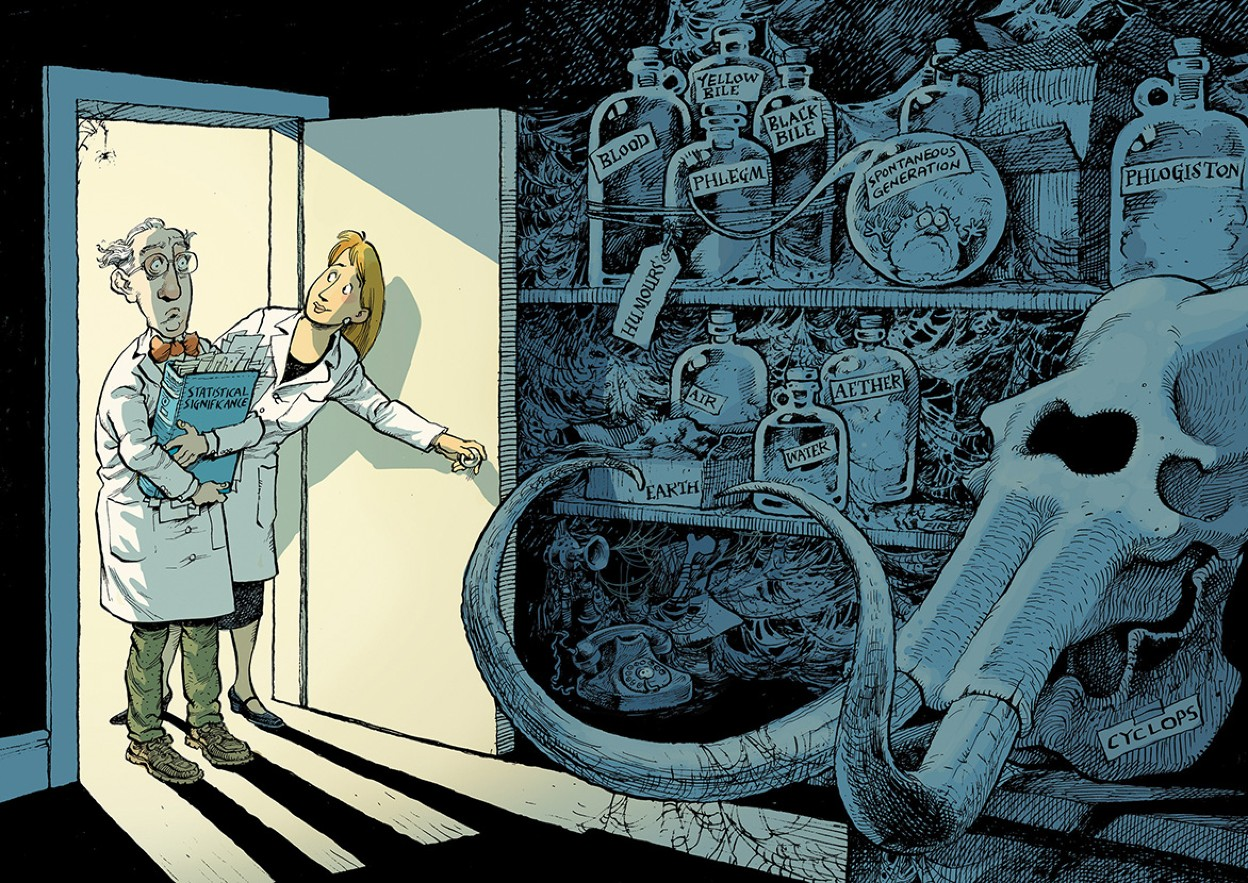
\includegraphics[width=.9\textwidth]{significance}
  \footnotesize
  \href{https://www.nature.com/articles/d41586-019-00857-9}{Amrhein et
    al. “Scientists rise up against statistical significance” 
    (2019)}
\end{frame}

\begin{frame}
  \frametitle{Нормальность и распределение слов}
  В парадигме стандартных статистических тестов при сравнении
  частотностей слов возникали проблемы:
  \begin{itemize}
  \item Предположение о нормальности неверно в случае частотного
    распределения слов
  \item В языке слишком много редких событий
  \item Неприменимость тестов, основанных на предположении о
    нормальности (напр., хи-кавдрат), как минимум к редким событиям (частотность < 5)
  \end{itemize}
\end{frame}

\begin{frame}
  \frametitle{Нормальное распределение излишне удивлено}
  \centering
  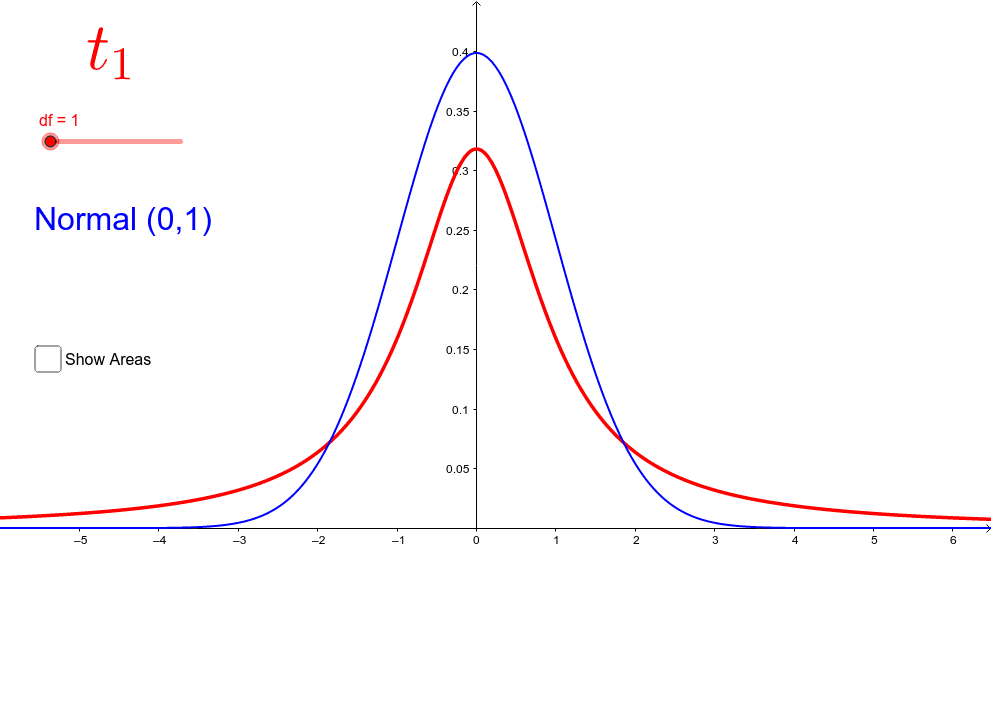
\includegraphics[width=\textwidth]{normal-student}
\end{frame}

\begin{frame}
  \frametitle{Отношение правдоподобия: мотивировка}
  \framesubtitle{Log likelihood ratio}
  Способ включить частотности слов в парадигму статистических тестов:

  \href{https://aclanthology.org/J93-1003.pdf}{Ted Dunning “Accurate
    Methods for the Statistics of Surprise and Coincidence” (1994)}
  \begin{itemize}
  \item Отношение правдоподобия менее зависит от предположения о
    нормальности распределения данных
  \item Поэтому не так резко завышает значимость редких событий и
    может применяться для оценки различий не только самых частотных слов
  \end{itemize}
\end{frame}

\begin{frame}
  \frametitle{Отношение правдоподобия: формула}
  \begin{tabular}[c]{|p{.3\textwidth}|c|c|c|}
    \hline
   & Корпус 1 & Корпус 2 & Всего \\
    \hline
    Частотность слова & a & b & a+b \\
    \hline
    Частотность остальных слов & c-a & d-b & c+d-a-b \\
    \hline
    Всего & c & d & c+d \\
    \hline
  \end{tabular}

\bigskip
  Ожидаемые частотности:
  \begin{itemize}
  \item[E1] $\frac{c}{c+d}(a+b)$
  \item[E2] $\frac{d}{c+d}(a+b)$
  \end{itemize}

  \begin{equation}
    LL = G^2 = 2 (a \log (a/E1) + b \log (b/E2) ) 
  \end{equation}
\end{frame}

\begin{frame}
  \frametitle{Проблема Log-Likelihood}
  \begin{itemize}
  \item Более чувствителен к частотным событиям (словам), чем к менее
    частотным [занижает степень различия по менее частотным словам]
  \end{itemize}
\end{frame}

\subsection{Взаимная информация}

\begin{frame}
  \frametitle{Условная вероятность}
$$
    P(Event|Condition)
$$
\end{frame}

\begin{frame}
  \frametitle{Условная вероятность}
  \begin{equation}
    P(B|A) = \frac{P(B \land A)}{P(A)}
  \end{equation}

  $$
    P(\text{интеллект}|\text{искусственный}) =
    \frac{P(\text{искусственный интеллект})}{P(\text{искусственный})}
    =$$

    $$
    = \frac{\frac{4}{46804371}}{\frac{121}{46804371}} = \frac{4}{121} = 0.033$$
\end{frame}

\begin{frame}
  \frametitle{Pointwise mutual information}
  \begin{columns}
    \column{.5\textwidth}
    PMI

  $$
  pmi(x;y) = log \frac{p(x,y)}{p(x)p(y)} =
  $$
  $$
  = log \frac{p(x|y)}{p(x)} =
  $$
  $$
  = log \frac{p(y|x)}{p(y)}
  $$

  Positive PMI

    $$
    ppmi(x;y) = max(pmi(x;y),0)
    $$    
    \column{.5\textwidth}
  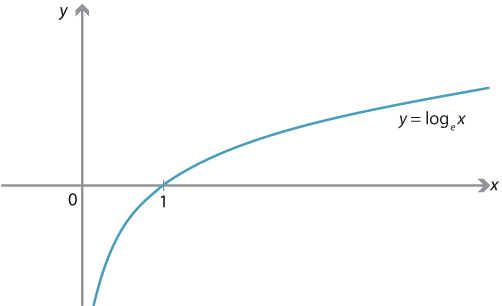
\includegraphics[width=\textwidth]{log}
  \end{columns}
\end{frame}

\begin{frame}
  \frametitle{Проблема PMI}
  \begin{itemize}
  \item Очень чувствителен к редким, но высоко информативным
    относительно друг друга событиям (слова встречаются всегда вместе)
    [завышает степень различия по редким словам]
  \end{itemize}
\end{frame}

\subsection{Байесовский подход}

\begin{frame}
  \frametitle{Вероятность независимых событий}
  Независимые события — наступление одного не изменяет вероятности
  другого.
  \begin{equation}
    P(B|A) = P(B) \quad | P(B) > 0
  \end{equation}

  \begin{equation}
    P(B \cap A) = P(A) \cdot P(B)
  \end{equation}
\end{frame}

\begin{frame}
  \frametitle{Совместная вероятность}
  \structure{Для независимых A и B}:

    $p(\text{A и B}) = p(A)p(B)$ \quad{} | $p(B|A) = p(B)$

    \bigskip

  \pause
  \structure{В общем случае}:

   $p(\text{A и B}) = p(A)p(B|A)$ \quad{} | $p(B|A) \neq p(B)$
\end{frame}

\begin{frame}
  \frametitle{Правило Байеса}
  \begin{equation}
    P(A|B) = \frac{P(B|A)P(A)}{P(B)}
  \end{equation}
  \pause
  \begin{equation}
    posterior = \frac{likelihood \cdot prior}{evidence}
  \end{equation}  
\end{frame}


\begin{frame}
  \frametitle{tidylo by Julia Silge: weighted log odds}
  \begin{enumerate}
  \item Log odds ratio:
    $$
    O_1 = \frac{f_{(w,c1)}}{N_{c1}-f_{(w,c1)}}
    $$
    $$
    O_2 = \frac{f_{(w,c2)}}{N_{c2}-f_{(w,c2)}}
    $$
    $$
    LO = log \frac{O_1}{O_2}
    $$
  \item Weighted by uninformative Dirichlet prior:
    $$
    \delta =
    \frac{\frac{f_{(w,c1)}+\alpha_{(w,c1)}}{N_{c1}+\alpha_{c1}-f_{(w,c1)}-\alpha_{(w,c1)}}}{\frac{f_{(w,c2)}+\alpha_{(w,c2)}}{N_{c2}+\alpha_{c2}-f_{(w,c2)}-\alpha{(w,c2)}}}
    $$
  \end{enumerate}
\end{frame}


\end{document}
